\FloatBarrier
\section{Anexos}

\subsection{Tablas de parámetros}

\begin{table}[H]
\centering
\caption{Condiciones de las corrientes de alimentación}
\label{tab:alimentacion}
\begin{tabular}{lcc}
\toprule
\textbf{Parámetro} & \textbf{Corriente azeotrópica} & \textbf{Solvente} \\
\midrule
Flujo [kmol/h] & 100 & 150 \\
Temperatura [$^\circ$C] & 47 & 47 \\
Presión absoluta [bar] & 3 & 3 \\
Composición molar & 0,5 -- 0,5 & 1 \\
\bottomrule
\end{tabular}
\end{table}


\begin{table}[H]
\centering
\caption{Condiciones de operación de las columnas}
\label{tab:operacion}
\begin{tabular}{lcc}
\toprule
\textbf{Parámetro} & \textbf{T-101} & \textbf{T-102} \\
\midrule
Presión absoluta [bar] & 1 & 1 \\
Flujo de destilado [kmol/h] & 50 & 50,5 \\
Razón de reflujo [mol/mol] & 1 & 0,5 \\
Número de etapas & 37 & 17 \\
Etapa de alimentación & 24 & 8 \\
Etapa de alimentación del agente separador & 4 & -- \\
\bottomrule
\end{tabular}
\end{table}


\begin{table}[H]
\centering
\caption{Parámetros de sintonización de controladores PI}
\label{tab:PI}
\footnotesize
\begin{tabularx}{\textwidth}{l *{6}{>{\centering\arraybackslash}X}}
\toprule
\textbf{Controlador} &
\textbf{Nivel de Condensador T-101} &
\textbf{Nivel de Rehervidor T-101} &
\textbf{Presión T-101} &
\textbf{Nivel de Condensador T-102} &
\textbf{Nivel de Rehervidor T-102} &
\textbf{Presión T-102} \\
\midrule

Ganancia (\%/\%) &
4,145 &
259,658 &
1,108 &
483,133 &
758,406 &
2,249 \\

Constante de tiempo $\tau$ [min] &
13,20 &
5,28 &
5,99 &
3,96 &
6,60 &
2,00 \\

\bottomrule
\end{tabularx}
\end{table}

\subsection{Figuras}

\begin{figure}[htbp]
    \centering
    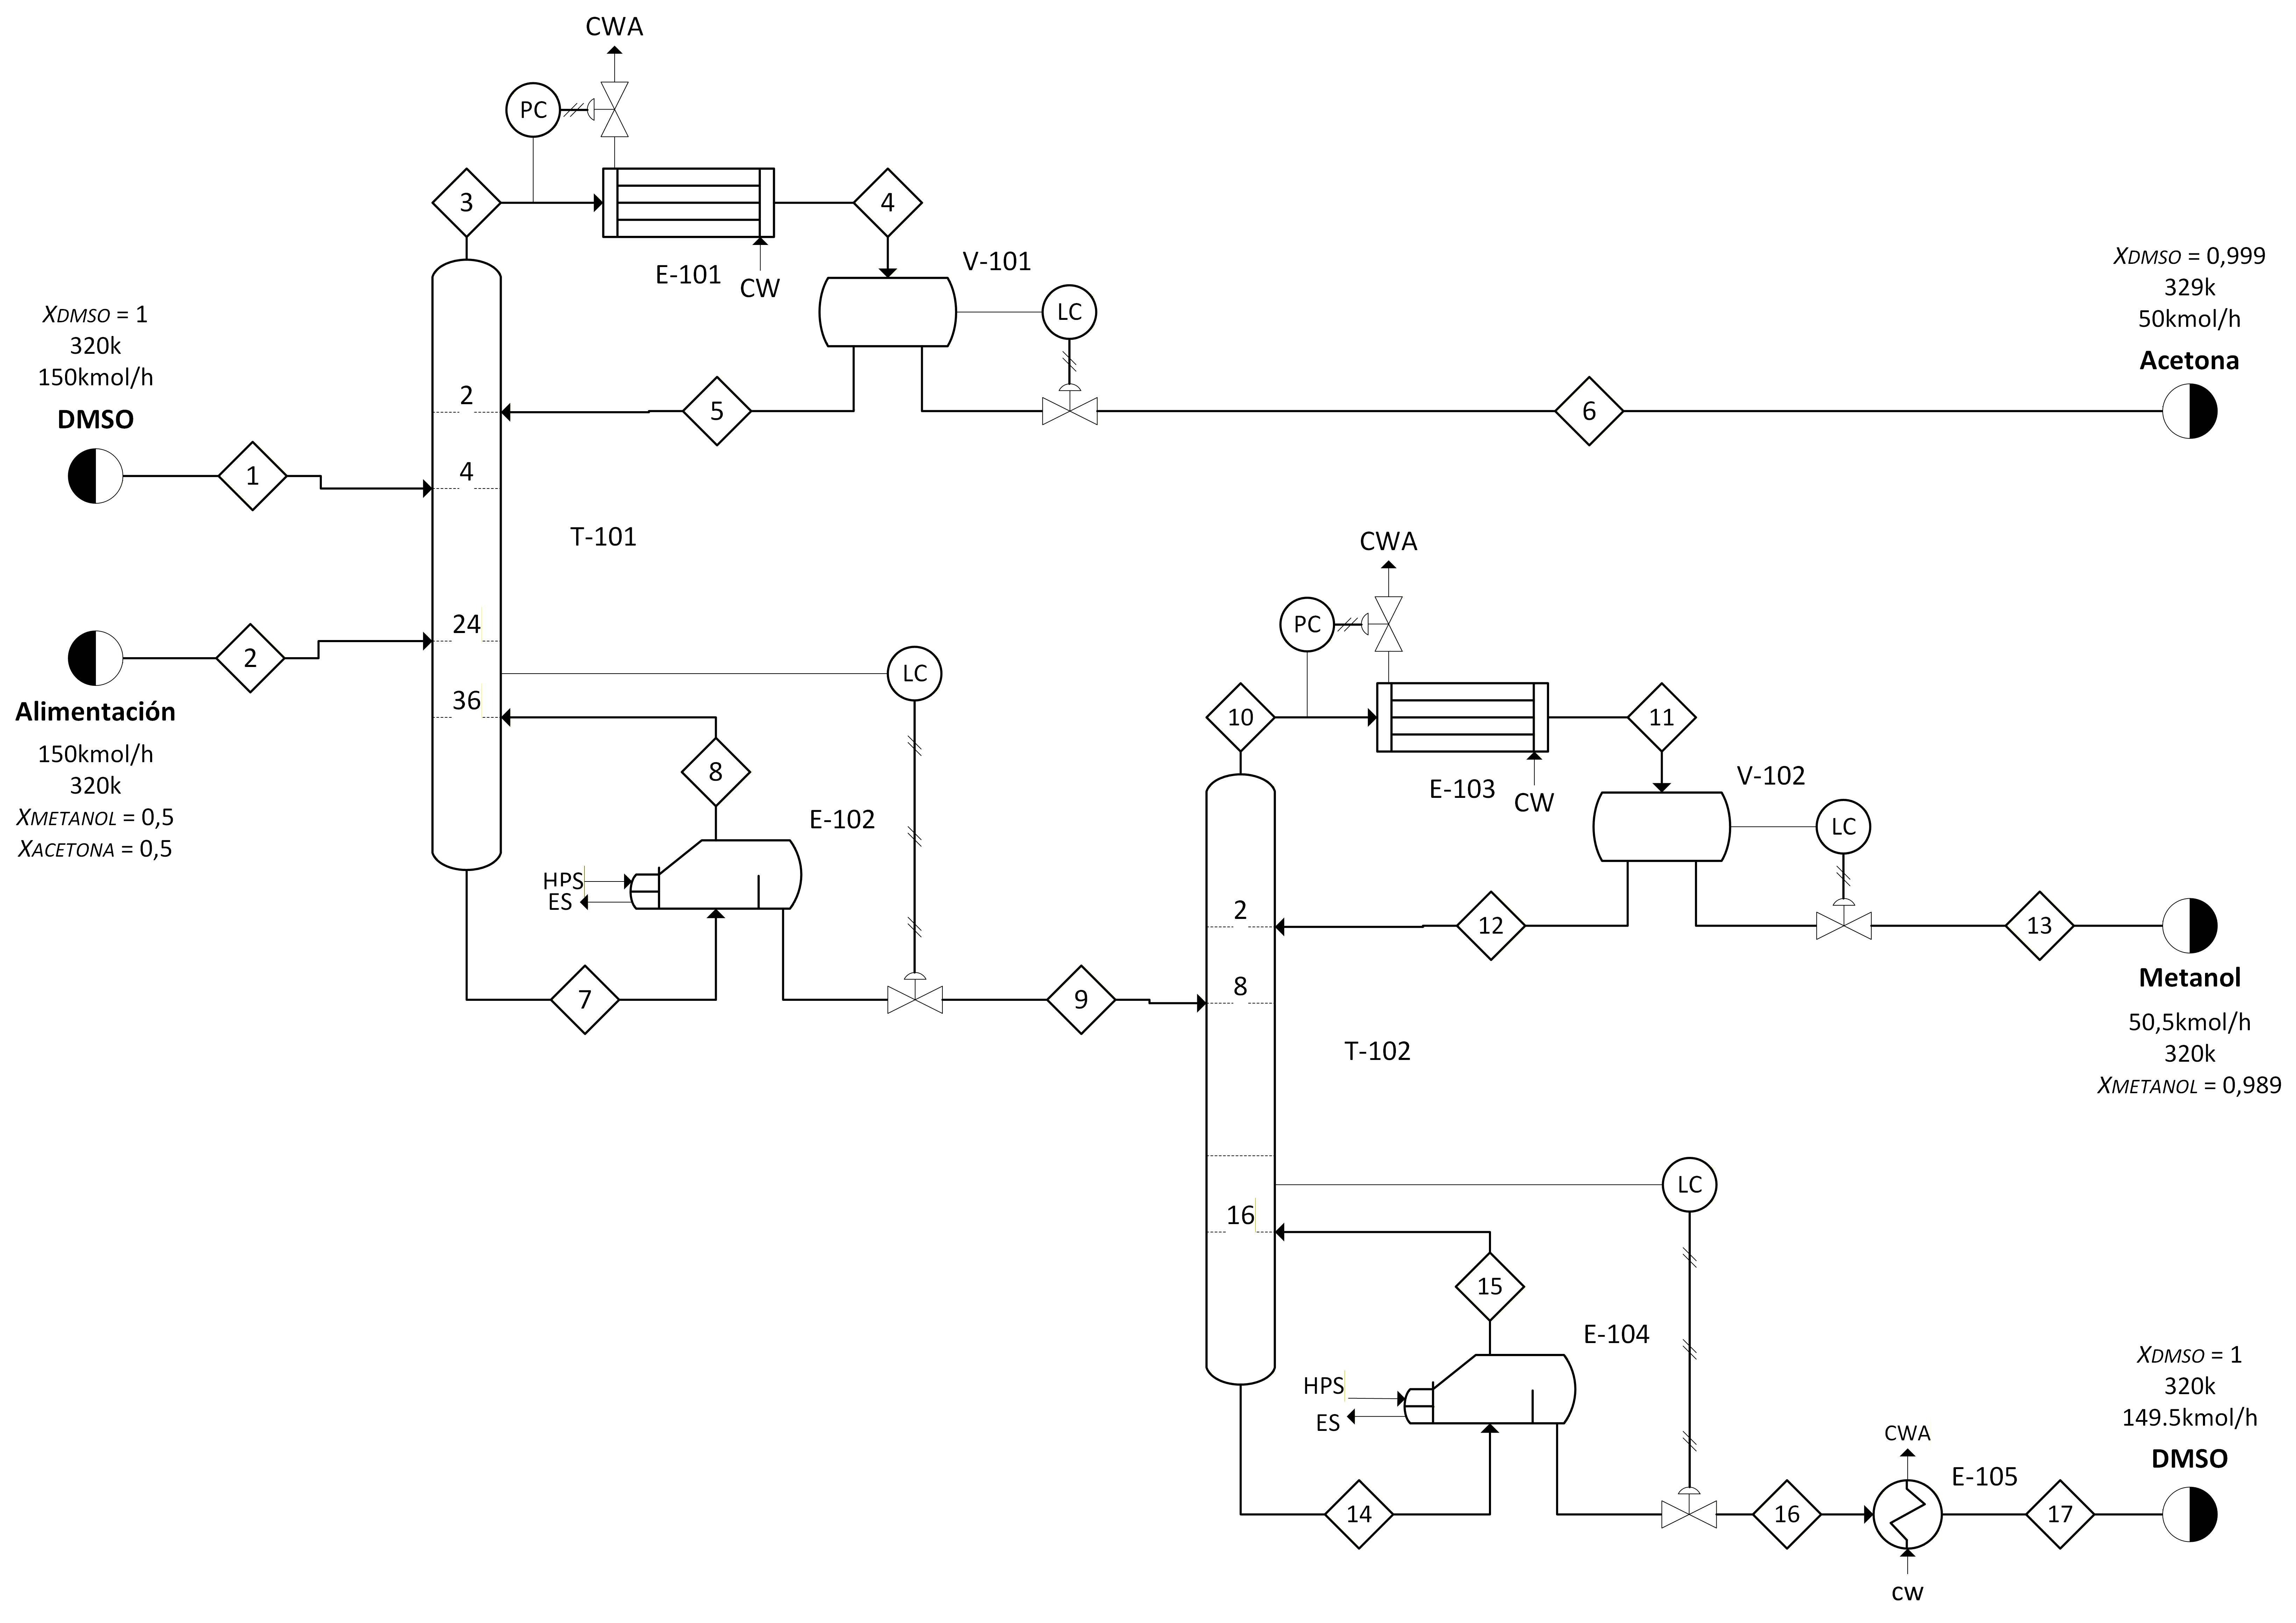
\includegraphics[width=1\textwidth]{figures/PFD_Tesis_2.jpg}
    \caption{Diagrama del proceso de destilación extractiva.}
    \label{fig:DiagramaPFD}
\end{figure}

\begin{figure}[htbp]
    \centering
    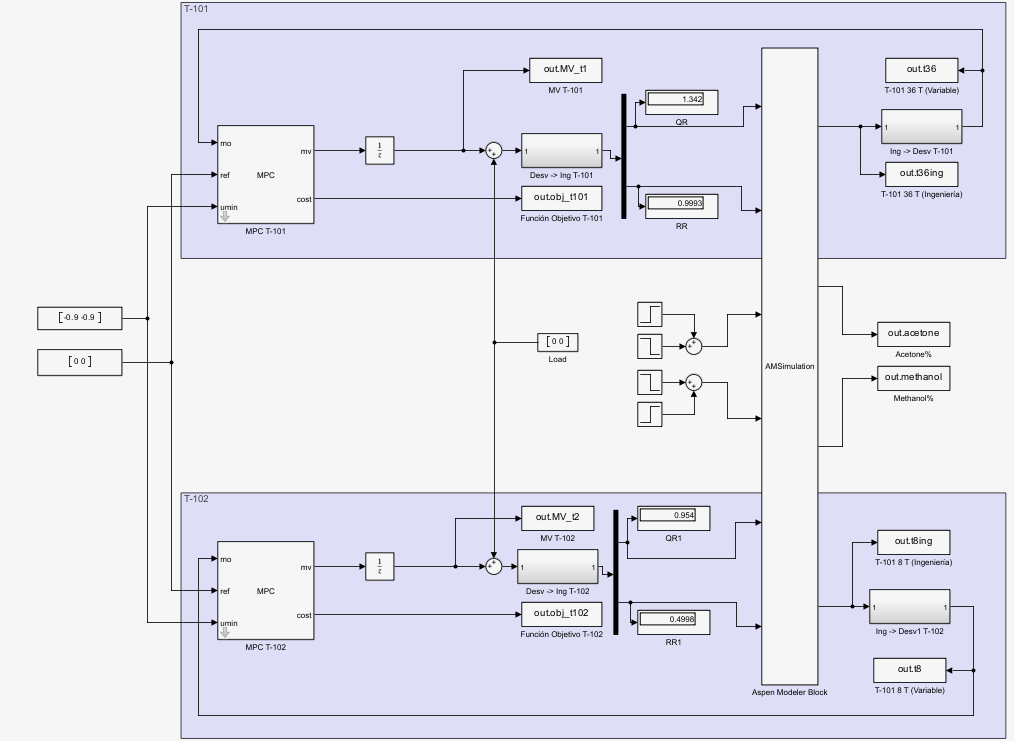
\includegraphics[width=1\textwidth]{figures/Simulink.png}
    \caption{Diagrama del control implementado en Simulink.}
    \label{fig:DiagramaSimulink}
\end{figure}

\begin{figure}[H]
    \centering
    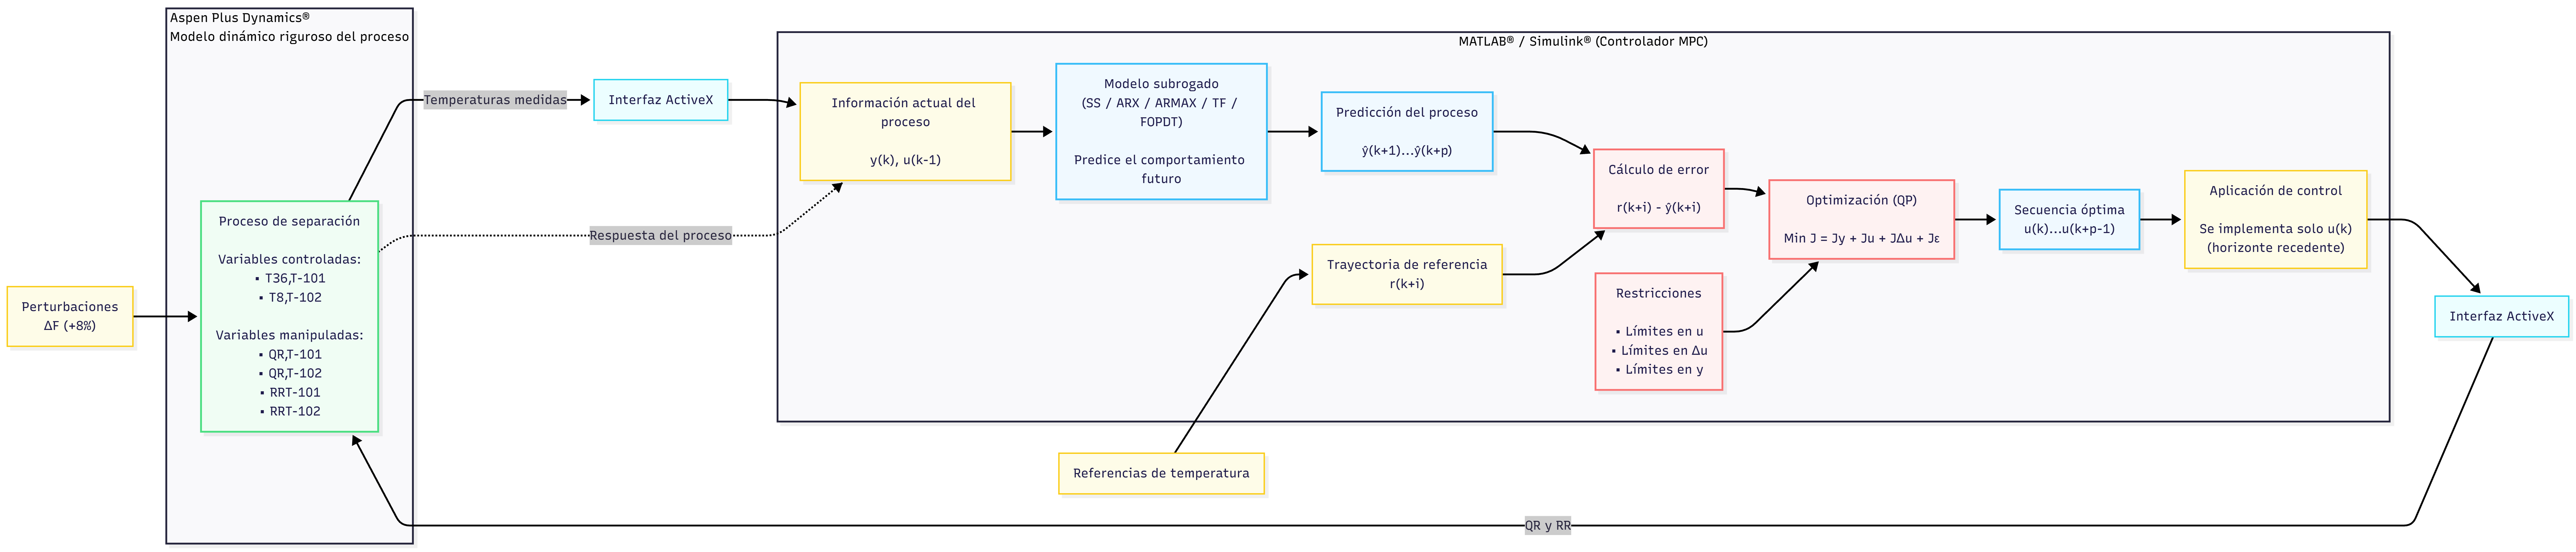
\includegraphics[width=1.00\textwidth]{figures/SIMULINK2.0.png}
    \caption{Esquema general del controlador MPC.}
    \label{fig:Simulink2.0}
\end{figure}

\FloatBarrier
\subsection{Parámetros de los metamodelos}

\begin{table}[H]
\centering
\caption{Parámetros de los modelos de espacio de estados}
\label{tab:SS_T101}
\scriptsize
\begin{tabular}{c c c c c}
\toprule
Estado & $A_i$ & $B_{1,i}$ & $B_{2,i}$ & $C_i$ \\

\midrule
\multicolumn{5}{c}{\textbf{SS-T101}} \\
\midrule


1 &
$[-41.655,\,-49.448,\,-11.960,\,9.380,\,\dots,\,26.246]$
& $-35.724$
& $-51.136$
& $-0.100$
\\

2 &
$[-5.326,\,-27.083,\,-9.948,\,9.762,\,\dots,\,29.930]$
& $36.406$
& $-25.489$
& $0.116$
\\

3 &
$[10.541,\,1.169,\,-3.682,\,10.149,\,\dots,\,23.047]$
& $37.626$
& $1.090$
& $-0.089$
\\

4 &
$[-2.281,\,-4.874,\,-5.059,\,-2.856,\,\dots,\,-24.919]$
& $-12.244$
& $-1.923$
& $-0.014$
\\

5 &
$[-3.141,\,-1.297,\,1.134,\,4.075,\,\dots,\,-21.496]$
& $-23.773$
& $0.404$
& $0.053$
\\

6 &
$[2.365,\,0.575,\,-1.673,\,-4.301,\,\dots,\,34.320]$
& $53.140$
& $-7.741$
& $0.013$
\\

7 &
$[-1.560,\,-1.509,\,-0.196,\,-1.116,\,\dots,\,-19.207]$
& $5.868$
& $-2.972$
& $0.001$
\\

8 &
$[0.473,\,1.124,\,1.055,\,0.045,\,\dots,\,22.195]$
& $14.265$
& $-3.948$
& $-0.009$
\\

9 &
$[0.046,\,1.309,\,1.704,\,4.322,\,\dots,\,-31.655]$
& $-61.955$
& $11.695$
& $-0.013$
\\

10 &
$[-3.113,\,-4.404,\,-1.517,\,-5.524,\,\dots,\,71.055]$
& $82.031$
& $-17.452$
& $-0.043$
\\

11 &
$[-0.695,\,-1.063,\,-0.714,\,-1.194,\,\dots,\,23.119]$
& $15.281$
& $-3.157$
& $-0.028$
\\

12 &
$[0.860,\,1.355,\,0.502,\,1.572,\,\dots,\,-29.076]$
& $-267.557$
& $59.473$
& $0.024$
\\

13 &
$[3.162,\,3.380,\,0.714,\,4.249,\,\dots,\,-307.461]$
& $-347.218$
& $67.553$
& $0.032$
\\

\midrule
\multicolumn{5}{c}{\textbf{SS-T102}} \\
\midrule

1 &
$[5.290,\,7.568,\,13.909,\,-1.207,\,\dots,\,-379.285]$
& $459.701$
& $-186.502$
& $-0.627$
\\

2 &
$[6.534,\,4.208,\,19.349,\,-0.231,\,\dots,\,-168.272]$
& $212.734$
& $-83.893$
& $0.411$
\\

3 &
$[-16.876,\,-22.461,\,-4.348,\,8.047,\,\dots,\,210.423]$
& $-300.916$
& $103.820$
& $0.069$
\\

4 &
$[10.072,\,9.761,\,-2.790,\,0.628,\,\dots,\,-343.757]$
& $431.665$
& $-164.476$
& $0.120$
\\

5 &
$[-12.012,\,-14.175,\,3.581,\,-16.123,\,\dots,\,368.584]$
& $-493.973$
& $183.489$
& $0.011$
\\

6 &
$[14.530,\,10.441,\,3.549,\,4.795,\,\dots,\,-378.990]$
& $523.556$
& $-195.367$
& $0.033$
\\

7 &
$[-13.793,\,-11.231,\,-6.545,\,1.252,\,\dots,\,325.515]$
& $-501.844$
& $170.494$
& $0.048$
\\

8 &
$[-2.810,\,-2.390,\,-1.212,\,0.593,\,\dots,\,93.562]$
& $-123.083$
& $47.610$
& $-0.807$
\\

9 &
$[-1.659,\,-0.068,\,-1.629,\,-0.456,\,\dots,\,36.076]$
& $-60.950$
& $27.741$
& $-0.043$
\\

10 &
$[0.574,\,0.682,\,0.160,\,-0.201,\,\dots,\,-23.202]$
& $36.153$
& $-14.139$
& $0.654$
\\

11 &
$[0.807,\,-0.032,\,0.606,\,0.480,\,\dots,\,-8.720]$
& $7.865$
& $-4.027$
& $0.853$
\\

12 &
$[-1.459,\,-0.762,\,-0.775,\,-0.357,\,\dots,\,32.508]$
& $-47.033$
& $18.620$
& $0.058$
\\

13 &
$[-2.253,\,-1.489,\,-1.114,\,-0.126,\,\dots,\,41.423]$
& $-64.506$
& $22.583$
& $-0.560$
\\

14 &
$[-0.288,\,-0.338,\,0.040,\,-0.068,\,\dots,\,12.602]$
& $-7.311$
& $2.070$
& $-1.404$
\\

15 &
$[0.575,\,0.360,\,0.254,\,0.058,\,\dots,\,-15.549]$
& $17.748$
& $-6.781$
& $-3.085$
\\

\bottomrule
\end{tabular}
\end{table}

\begin{table}[H]
\centering
\caption{Parámetros de modelos de subrogación para T-101}
\label{tab:T101}
\footnotesize
\begin{tabularx}{\textwidth}{l c >{\raggedright\arraybackslash}p{0.75\textwidth}}
\toprule
\textbf{Modelo} & \textbf{Entrada} & \textbf{Parámetros} \\
\midrule

ARX-T101 & -- &
$A = [1.000,\,-1.356,\,0.200,\,-0.001,\,0.119,\,0.080,\,0.005,\,-0.028,\,-0.030,\,-0.001,\,0.010]$ \\
& & $B_1 = [0.000,\,0.164,\,-0.158,\,-0.027,\,-0.009,\,0.012,\,0.018,\,0.010,\,0.002,\,-0.009,\,-0.002,\,0.002,\,0.001,\,0.001,\,-0.003]$ \\
& & $B_2 = [0.000,\,0.004,\,-0.041,\,0.040,\,0.000,\,0.001,\,-0.003,\,-0.004,\,-0.001,\,0.001,\,0.002,\,0.001]$ \\[0.4em]

ARMAX-T101 & -- &
$A = [1.000,\,-3.882,\,5.962,\,-4.459,\,1.470,\,0.033,\,-0.176,\,0.086,\,-0.051,\,0.028,\,-0.022,\,0.019,\,-0.013,\,0.006,\,-0.001]$ \\
& & $B_1 = [0.000,\,0.164,\,-0.572,\,0.755,\,-0.438,\,0.065,\,0.045,\,-0.021,\,0.006,\,-0.011,\,0.017,\,-0.014,\,0.004,\,0.001]$ \\
& & $B_2 = [0.000,\,0.004,\,-0.051,\,0.153,\,-0.199,\,0.125,\,-0.028,\,-0.008,\,0.008,\,-0.004,\,0.001]$ \\
& & $C = [1.000,\,-2.530,\,2.345,\,-0.789,\,-0.185,\,0.165]$ \\[0.4em]

TF-T101 & -- &
$b_{z1} = [3820.400,\,17617.000]$ \\
& & $b_{z2} = [-34.711,\,-14016.000]$ \\
& & $a_{p1} = [1.000,\,212.299,\,10892.000,\,50753.000]$ \\
& & $a_{p2} = [1.000,\,77.591,\,5064.300,\,181330.000]$ \\
& & $\tau_{1} = 1,\qquad \tau_{2} = 2$ \\[0.4em]

FOPDT-T101 & -- &
$K_{p1} = 0.358,\qquad K_{p2} = -0.079$ \\
& & $\tau_{1} = 0.125,\qquad \tau_{2} = 0.203$ \\
& & $\theta_{1} = 0.000,\qquad \theta_{2} = 0.050$ \\[0.4em]

\bottomrule
\end{tabularx}
\end{table}

\begin{table}[H]
\centering
\caption{Parámetros de modelos de subrogación para T-102}
\label{tab:T102}
\footnotesize
\begin{tabularx}{\textwidth}{l c X}
\toprule
\textbf{Modelo} & \textbf{Entrada} & \textbf{Parámetros} \\
\midrule

ARX-T102 & -- &
$A = [1.000,\,-1.753,\,0.895,\,-0.168,\,0.210,\,-0.086,\,-0.286,\,0.247,\,-0.064,\,0.068,\,-0.100,\,0.028,\,0.013,\,-0.010,\,0.005]$ \\
& & $B_1 = [0.000,\,0.310,\,-0.410,\,0.086,\,0.017,\,0.115,\,-0.001,\,-0.169,\,0.049,\,0.014,\,0.037,\,-0.037,\,-0.010]$ \\
& & $B_2 = [0.000,\,-0.036,\,0.054,\,-0.020,\,0.003,\,-0.011,\,-0.012,\,-0.001,\,0.022,\,0.007,\,-0.010,\,-0.003,\,0.002,\,0.006]$ \\[0.4em]

ARMAX-T102 & -- &
$A = [1.000,\,-2.548,\,2.294,\,-0.909,\,0.157,\,0.042,\,-0.090,\,0.110,\,-0.098,\,0.072,\,-0.047,\,0.018,\,0.002,\,-0.002,\,-0.001]$ \\
& & $B_1 = [0.000,\,0.310,\,-0.657,\,0.414,\,-0.060,\,0.040,\,-0.028,\,-0.096,\,0.094,\,-0.028,\,0.020,\,-0.009]$ \\
& & $B_2 = [0.000,\,-0.036,\,0.082,\,-0.063,\,0.021,\,-0.007,\,-0.012,\,0.003,\,0.033,\,-0.012,\,-0.011,\,0.004,\,-0.002,\,0.000]$ \\
& & $C = [1.000,\,-0.800,\,0.014,\,-0.025,\,-0.239,\,-0.092,\,0.199]$ \\[0.4em]

TF-T102 & -- &
$b_{z1} = [-12642.000,\,573210.000]$ \\
& & $b_{z2} = [-765.156,\,-29177.000]$ \\
& & $a_{p1} = [1.000,\,104.584,\,16107.000,\,581590.000]$ \\
& & $a_{p2} = [1.000,\,214.425,\,9192.300,\,261610.000]$ \\
& & $\tau_{1} = 1,\qquad \tau_{2} = 1$ \\[0.4em]

FOPDT-T102 & -- &
$K_{p1} = 1.010,\qquad K_{p2} = -0.113$ \\
& & $\tau_{1} = 0.222,\qquad \tau_{2} = 0.255$ \\
& & $\theta_{1} = 0.000,\qquad \theta_{2} = 0.000$ \\[0.4em]

\bottomrule
\end{tabularx}
\end{table}
